\subsection{Breaking Down the Challenge}
\label{sec:flight}
Any aircraft participating in the UAV Challenge must be autonomous, only interacting with a human to be armed or disarmed at the beginning and end of the mission. In order to develop 
The Medical Express mission can be broken down into three discrete flight maneuvers:
\begin{enumerate}[label=\bfseries M\arabic*:] \itemsep-2pt
	\item Vertical take-off to cruising height, and landing
	\item Fixed-wing flight, navigating through waypoints and keeping within GeoFence boundaries
	\item Aerial search
\end{enumerate}

Using these maneuvers, completing the mission can be described as completing the sequence of actions\\
\begin{tabular}{r l l}
	1. & Mission start after being armed & (\textbf{M1}) \\ 
	2. & Navigate to Joe's location & (\textbf{M2}) \\ 
	3. & Aerial search to identify Joe & (\textbf{M3}) \\ 
	4. & Land near Joe to collect blood & (\textbf{M1}) \\ 
	5. & Take-off after being re-armed & (\textbf{M1}) \\ 
	6. & Navigate back to base & (\textbf{M2}) \\ 
	7. & Land at base & (\textbf{M1}) \\ 
\end{tabular} 

\subsection{Development}
Figure \ref{fig:softwarearchitecture} shows the autonomous flight and intelligence architecture implemented on the aircraft.

\red{Considerations:
	
	time cost -> prototype style / separate each module (allows cut off were we get to with some functionality)
	Extendibility -> for future years
	Concurrency -> Multiprocessing
	Latency -> processes polling / non blocking io etc
}

\red{Autonomy on Raspberry Pi}

\red{\begin{itemize}
	\item Generation of flight path, currently from text file but ideally based on sensing (flight.py)
	\item Capability for executing known/expected commands by sending to PixHawk (autopilot.py)
	\item Monitoring status of aircraft such as position, velocity (uavstate.py)
	\item Monitoring status of world such position of obstacles, waypoints (worldstate.py)
	\item Logging of flight conditions, sensing and motion (logging.py)
	\item Unsure what interface.py does
\end{itemize}}

\begin{figure}[!ht]
	\centering
	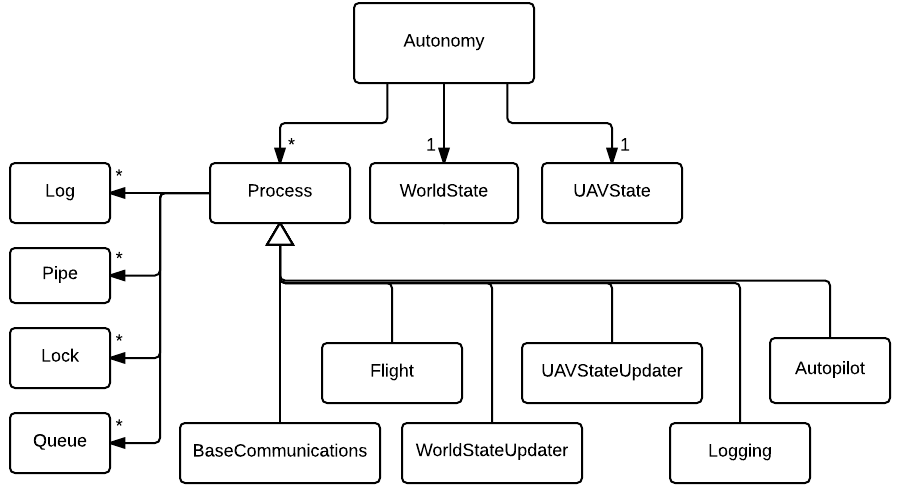
\includegraphics[width=350pt]{\IMAGEPATH /Diagrams/software}
	\caption{High level software architecture}
	\label{fig:softwarearchitecture}
\end{figure}

\subsection{Testing}
\red{Software in the Loop}

\begin{figure}[!ht]
	\centering
	\includegraphics[width=200pt]{\IMAGEPATH emblem}
	\caption{Software in the Loop testing}
	\label{fig:sitl}
\end{figure}